
%darc, the Durham Adaptive optics Real-time Controller.
%Copyright (C) 2010 Alastair Basden.

%This program is free software: you can redistribute it and/or modify
%it under the terms of the GNU Affero General Public License as
%published by the Free Software Foundation, either version 3 of the
%License, or (at your option) any later version.

%This program is distributed in the hope that it will be useful,
%but WITHOUT ANY WARRANTY; without even the implied warranty of
%MERCHANTABILITY or FITNESS FOR A PARTICULAR PURPOSE.  See the
%GNU Affero General Public License for more details.

%You should have received a copy of the GNU Affero General Public License
%along with this program.  If not, see <http://www.gnu.org/licenses/>.

\documentclass[a4,10pt]{article}
\providecommand{\gitID}{$Id: 220a431836ba0173bbffee0c5f7c5bcc1bfc720f $}
\usepackage[pdftex,pagebackref=true,colorlinks=true,linkcolor=blue]{hyperref}
\usepackage{xspace}
\usepackage{graphicx}
\newcommand{\ao}{adaptive optics (AO)\renewcommand{\ao}{AO\xspace}\xspace}
\newcommand{\cpu}{central processing unit
  (CPU)\renewcommand{\cpu}{CPU\xspace}\xspace}
\newcommand{\rtcs}{real-time control system (RTCS)\renewcommand{\rtcs}{RTCS\xspace}\xspace}
\newcommand{\dm}{deformable mirror (DM)\renewcommand{\dm}{DM\xspace}\xspace}
\newcommand{\wfs}{wavefront sensor (WFS)\renewcommand{\wfs}{WFS\xspace}\xspace}
\usepackage{amsmath}
\newcommand{\ignore}[1]{}
\title{darc: Developers guide}
\author{Alastair Basden \\ a.g.basden@durham.ac.uk \\ Durham University \\ Department of Physics
  \\ South Road \\ Durham \\ DH1 3LE \\ UK}


\setlength{\textheight}{21.5cm}%
\setlength{\textwidth}{18cm}%
\setlength{\hoffset}{-3.0cm}%
\setlength{\footskip}{1.5cm}%
\setlength{\headsep}{2.5cm}%
\setlength{\voffset}{-2.5cm}%

\begin{document}
\maketitle
{\hspace{7cm} 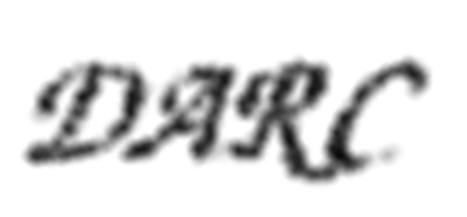
\includegraphics[width=3cm]{darclogo.eps}}
\vfill
\gitID
%\section{Quickstart guide}
%%darc, the Durham Adaptive optics Real-time Controller.
%Copyright (C) 2010 Alastair Basden.

%This program is free software: you can redistribute it and/or modify
%it under the terms of the GNU Affero General Public License as
%published by the Free Software Foundation, either version 3 of the
%License, or (at your option) any later version.

%This program is distributed in the hope that it will be useful,
%but WITHOUT ANY WARRANTY; without even the implied warranty of
%MERCHANTABILITY or FITNESS FOR A PARTICULAR PURPOSE.  See the
%GNU Affero General Public License for more details.

%You should have received a copy of the GNU Affero General Public License
%along with this program.  If not, see <http://www.gnu.org/licenses/>.

\begin{verbatim}
QUICKSTART for Paris, Oct 2009

To get the system into a working 2 camera mode:

Plug monitor and keyboard into telemetry server (small HP machine)
Network cable (motherboard) to your external network.
Network cable (PCI) to the local switch.
You will need to configure this machine for external network access.


Boot the telemetry server (small HP machine).
Wait until it has booted (5 minutes to allow crontab time to run).
It logs on automatically.
Open a terminal.
cd /Canary/rtc
./recvStream.py


Plug Network cable on camera PC (black dell machine) into the switch.
Plug the camera fibre into the right hand port.
Plug the camera trigger for the 2 cameras into the cameras and into
the two right hand BNC connectors.
Boot the camera PC (black Dell machine)

Plug network cable on RTC PC (mac pro) into port 1, and into the switch.
Plug the camera fibre into port 0 (right hand port).

Boot the RTC (mac pro).
Log into the RTC as canary twice (ssh from the telemetry server: ssh -X rtc ).
In each, type:
source /Canary/etc/rtc.bashrc
In one type:
cd rtc
./control.py

In the other type:
cd rtc
./startStreams.py -h192.168.0.1

Note - eventually, this should be self-starting, but when we changed
the network config just before shipping it stopped working, so please
do it manually for now.


On the telemetry server, 
open a terminal and type:
cd /Canary/rtc
./rtcgui.py


Make sure that you have a suitable config file (e.g. config2camera.py
or configshakti.py) in /Canary/rtc/ on the telemetry server and in
/home/canary/rtc/ on the rtc machine (mac pro).  

This is currently a bug, which will be fixed (we didn't want to fix it
in the hour before shipping!).

On the GUI, click the start button.  Choose the config file
config2camera.py.  The RTC should then start running.

If working in 1 camera mode, use configshakti.py.

Go to the streams tab, and turn on some streams.  
For example put 100 100 100 in the 3 entry boxes next to rtcPxlBuf.
This sets the decimate rates (for this GUI, out of the RTC between RTC
and tememetry server).
Do this for rtcPxlBuf

Click the spawn plot button.
Select the rtcPxlBuf button in the subscribe too... window, then close
the subscribe too... window.

This will then start showing camera pixels.
To view as an image, type into the text entry box in the bottom left
of the plot:
data.shape=128,256
and then click elsewhere on the screen (so that
the text entry looses focus).
This will show interleaved camera data.
To view from just one camera do either:
data.shape=128,256
data=data[:,::2]
or
data.shape=128,256
data=data[:,1::2]

Any valid python code can be inserted here.  It can be used for
implementing overlays or anything else you wish.

Note, to avoid having to do this, you can set up some plots, and save
them to a configuration file.  Some examples have been done for you -
run the GUI with:
./rtcgui.py initPhaseA.py
A list of available plots then appears in the GUI.
(some of these will work with 2 camera mode, some with 1 camera mode).
These can then be toggled to display or remove plots.

Feel free to edit initPhaseA.py as you wish.

To run some test scripts (some examples of how to do things with the camera):
cd /Canary/local/scripts/test
and look at these scripts.

Note - if any of these scripts require rtc output (pixels/slopes etc),
then the streams need to be turned on in the GUI first, as the script
facility to turn streams on hasn't been implemented yet.


\end{verbatim}


\pagebreak
\tableofcontents
\pagebreak
\section{License}
darc, the Durham Adaptive optics Real-time Controller.
Copyright (C) 2010 Alastair Basden.

This program is free software: you can redistribute it and/or modify
it under the terms of the GNU Affero General Public License as
published by the Free Software Foundation, either version 3 of the
License, or (at your option) any later version.

This program is distributed in the hope that it will be useful,
but WITHOUT ANY WARRANTY; without even the implied warranty of
MERCHANTABILITY or FITNESS FOR A PARTICULAR PURPOSE.  See the
GNU Affero General Public License for more details.

You should have received a copy of the GNU Affero General Public License
along with this program.  If not, see <http://www.gnu.org/licenses/>.

The lead author has a preference that darc should not be used for
military purposes or by organisations with military connections,
however this is not enforceable due to the open nature of the license.

\section{Introduction}
darc, the Durham adaptive optics real-time controller is a generic
controller for adaptive optics systems, and can be configured and
adapted for use with almost any such system.  It has been designed
with low latency as a primary consideration, allowing high performance
\ao to be achieved, with many adjustable parameters being available to
tailor the performance of darc to given hardware and a given \ao
system.

darc was initially designed as a proof of concept to demonstrate that
\cpu based processing on modern processors was sufficient for small
and medium sized \ao systems, negating the need for complex hardware
and long development times.  The success of this demonstration was
such that after some rationalisation and tidying up, darc was made
publicly available.

\subsection{Document purpose}
The purpose of this document is to aid developers of darc:  those who
need to develop one or more components to meet their requirements.
This will include those who are developing camera or \dm interface
modules, those who need to interface darc with a telescope (or other
instrument) control system, and those who require a different
telemetry interface.  It will also include those developing new
algorithms for darc, and those seeking to use darc for new purposes.

This document is not intended for general users of darc who require
only knowledge of how to operate the system.

This document lays out the various different parts of darc that are
open for development, and provides hints and advise on how these can
be developed to meet specific requirements.

\section{darc components overview}
\subsection{darc core structure}
darc is optimised for astronomical \ao real-time control, delivering
low latency and high frame rates.  A horizontal processing strategy
(Fig.~\ref{fig:horiz}) is key to this, minimising inter-thread
communication, and allowing good load balancing.  Here, each
sub-aperture is processed by a single thread from pixel calibration,
to slope calculation and finally partial wavefront reconstruction.  

\begin{figure}
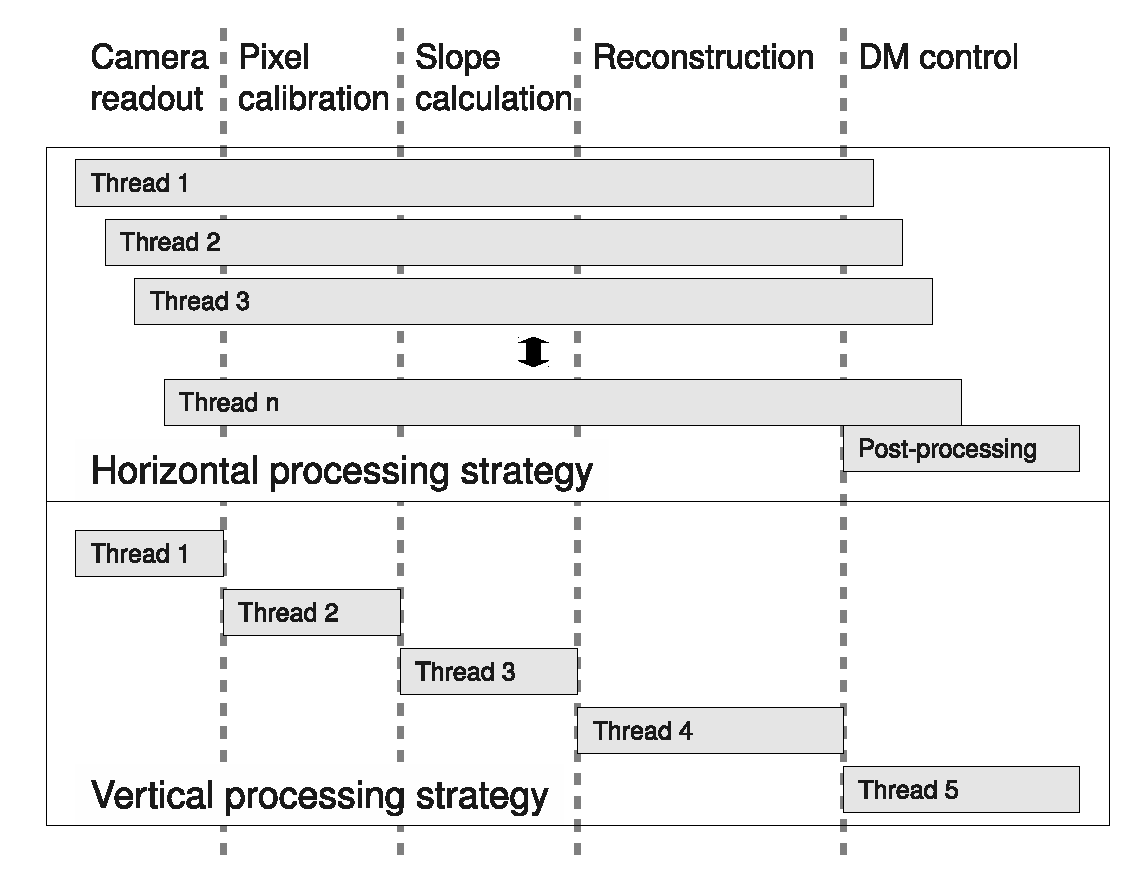
\includegraphics[width=0.5\linewidth]{processingStrategy.eps}
\caption{Horizontal processing strategy used by
  darc (above), contrasted with a more conventional vertical
  processing strategy.}
\label{fig:horiz}
\end{figure}

\subsubsection{darc modules}
darc has a modular design allowing different parts to be replaced and
developed on the fly.  Modules exist for:
\begin{itemize}
\item Camera interfaces (e.g.\ camfile.c, sl240Int32cam.c, camv4l.c,
  camuEyeUSB.c).
\item \dm interfaces (e.g.\ mirrorAdaptica64.c, mirrorBMMMulti.c,
  mirrorSocket.c).
\item Image calibration (e.g.\ rtccalibrate.c).
\item Slope calculation (e.g.\ rtcslope.c).
\item Wavefront reconstruction (e.g.\ reconmvm.c, reconLQG.c).
\item On-the-fly parameter buffer update (e.g.\ rtcbuffer.c).
\end{itemize}
The filenames here are found within the {\tt src/} directory of the
darc source code tree.  These modules are dynamically loadable,
allowing changes to be made while the system is in operation.

Development of these modules is in C.

\subsection{darc control}
Control of darc is performed by writing to a double buffered shared
memory region ({\tt /dev/shm/rtcParam1 and /dev/shm/rtcParam2}), which
the core darc real-time pipeline then reads.  The standard way of
controlling darc is via the control program, which is written in
Python.  However, alternative control techniques can be developed in
any language which can access shared memory and has access to Posix
mutexes and condition variables.

The standard control program, {\tt control.py}, is used to set and get
parameters within the darc shared memory regions.  This program also
has interfaces that make it accessible to clients.  Currently, there
are two options available, using middleware based on CORBA or Pyro.
These serve as examples, and it is possible to other other middleware
options as desired.

A darc module interface is also available to allow the parameters to
be updated on a frame-by-frame basis.  However, this is highly
specific and not considered further here.

\subsubsection{Configuration}
darc is configured initially using a parameter file, which can be
either Python or FITS (using the default control program).  

\subsection{darc telemetry}
Telemetry in darc refers to data that changes rapidly, is produced by
the real-time control system, and is useful for operations such as
determining system state, viewing information and as an aid for
control.  Examples of telemetry include \wfs pixel information, \dm
commands and slope measurements, all of which will be produced
rapidly, depending on \ao system frame rate.  These are referred to as
{\em telemetry streams}, and in the standard darc configuration,
several default streams are available, including
\begin{itemize}
\item Raw pixels
\item Calibrated pixels
\item Wavefront slopes
\item Wavefront flux
\item Reconstructed phase
\item DM commands
\item Status
\item Errors
\end{itemize}

Additional telemetry streams can be added by developing darc modules
that export the desired information.

Telemetry streams are implemented using shared memory circular
buffers, which the real-time core writes information to, allowing
clients to read this information (usually, though not exclusively)
through the control program.  The rate at which data should be written
to these buffers is written (and modifiable) within the header of the
circular buffer.  A time stamp and frame number is also written to
each entry of the circular buffers.

Telemetry information is delivered to clients (local and remote) using
a telemetry back-end.  As with most darc components, this is modular,
and can easily be replaced by the system developer.  The default
back-end relies on TCP/IP sockets with a receiver process for each
stream required on the client host, and a sender process required on
the PC running darc.  This provides a simple, easily understandable
transport medium, but one which is not ideal when the data-rate
becomes high.  At this point, alternative transport mediums should be
considered.  It should be noted that data is only send once to each
host, not once to each client.  Once data arrives at a host, it is
written to a shared memory circular buffer which the clients are then
free to use.

All telemetry information is delivered as a 1D array of data.  It is
up to the client to determine how this should be interpreted.

\subsubsection{Real-time displays}
darc is provided with a real-time display interface which can be used
to display telemetry information in both 1D and 2D formats.  These
displays are generic, but can be configured to display data in a
particular way using a configuration file, or on the fly by entering
Python commands to reformat the data.

\subsection{darc directory structure}
The darc source repository has the following directories:
\begin{itemize}
\item {\bf bin/}  Applications (Python and compiled).
\item {\bf conf}  Example configuration scripts, for both darc
  parameter files and real-time displays.
\item {\bf doc/}  Documentation (requires compiling).
\item {\bf etc/}  Example environment files.
\item {\bf idl/}  Interface definition for the darc CORBA interface.
\item {\bf include/}  Include header files for module development.
\item {\bf lib/}  Compiled libraries, including darc modules.
\item {\bf lib/python/} Python libraries.
\item {\bf src/}  Source code for darc and standard interface modules.
\item {\bf test/} Scripts and data for performing tests.
\end{itemize}

Within the top level directory there is a Makefile, a README and
INSTALL file.

Upon a {\tt make install} command, darc is installed in {\tt /opt/darc} by
default.  However, this can be altered by creating a
{\tt Makefile.config.local} file which customises the values found in
{\tt Makefile.config}.


\section{Development of darc core modules}
To develop a darc core module (algorithm or camera/\dm interface),
selected functions provided within a header file must be filled out,
and a shared object library created.  It is not necessary to provide
all of these functions, providing flexibility for different requirements.

In general, the available functions are
\begin{itemize}
\item Open:  Required, to initialise the module.
\item Close: Required, to finalise/free the module.
\item NewParam: Optional, to access the darc parameter buffer (not all
  modules require access to parameters).
\item NewFrame: Optional, called at the start of a new frame by the
  init/finalisation thread.
\item NewFrameSync: Optional, called once at the start of a new frame,
  by a sub-aperture processing thread.
\item StartFrame:  Optional, called once per sub-aperture processing
  thread at the start of each frame.
\item Process: Optional, called once for each sub-aperture,
  ideally where the main processing is done (for example, image
  calibration, or slope computation, or partial reconstruction).
\item EndFrame: Optional, called once sub-aperture processing thread
  at the end of each frame.
\item FrameFinishedSync: Optional, called once per frame by a
  sub-aperture processing thread.
\item FrameFinished: Optional, called once per frame, by a
  non-sub-aperture processing thread.
\item OpenLoop: Optional, called if the \ao loop is open (to allow
  reset of parameters).
\item Complete: Optional, called after everything has been completed,
  by a non-sub-aperture processing thread.
\end{itemize}

These call points are shown in Fig.~\ref{fig:hooks}.  It is up to the
module developer to determine which functions they require.  This can
be based on the requirements of existing modules.  The large number of
available functions means that darc is very flexible, and although
geared towards processing of data on a per-sub-aperture basis (for
example like a Shack-Hartmann or Pyramid based \ao system), this is
not necessary, and it can be used for flexible real-time processing of
most algorithms.

\begin{figure}
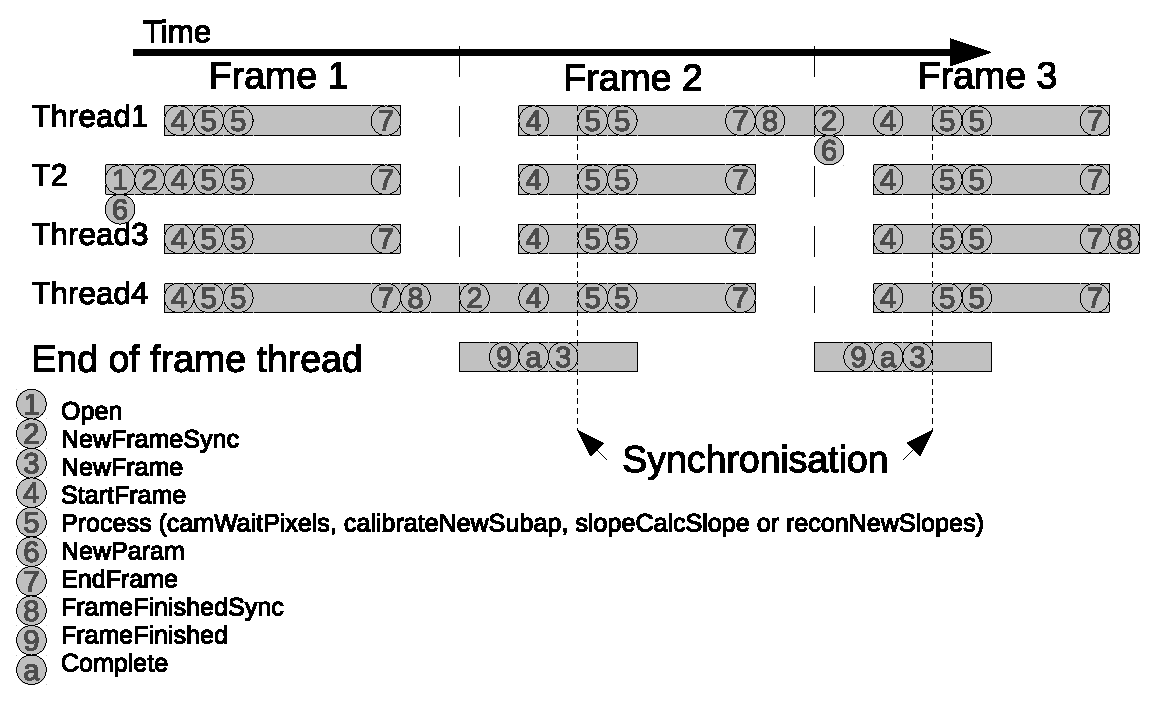
\includegraphics[width=0.5\linewidth]{hooks.eps}
\caption{The module interface function call points during several
  frames of real-time operation.}
\label{fig:hooks}
\end{figure}

The exact function definitions for these modules are found in the {\tt
  include/} directory, and examples from the {\tt src/} directory can
be followed.

\subsection{Accessing the parameter buffer}
The darc parameter buffer has a rather obtuse layout, designed to
optimise the real-time process.  As a developer, you will only need to
know about this if developing a new control interface.  In that case,
details are provided in {\tt lib/python/buffer.py} and in {\tt src/buffer.c}
and {\tt include/buffer.h}.

\section{Development of a new control interface}
If you are unable to use Python in your project, it will be necessary
to develop a new control interface.  For basic functionality, this is
fairly trivial since all that is required is to write data to a shared
memory region.  However, an understanding of the layout of this memory
region is required, and should be gained by investigating the relevant
source files, including {\tt lib/python/buffer.py}, {\tt src/buffer.c}
and {\tt include/buffer.h}.

You may also wish this control interface to provide control for the
telemetry sub-system too, and this can be developed depending on your
requirements.

\subsection{Alternative middleware}
If you wish to implement control of darc using your own middleware
(i.e.\ not CORBA or Pyro), then you must develop a new control
interface.  The simplest way to do this is to copy the existing
{\tt control.py}, {\tt controlCorba.py}, {\tt controlPyro.py} and {\tt
  controlVirtual.py} found in {\tt lib/python}.  However, if Python
does not have a suitable interface to your selected middleware, or if
you do not wish to use Python, the task will be more involved, though
far from impossible.

\subsection{Control requirements}
The default control functionality is described here, and at least some
of this will require translating to your requirements, though by no
means all.

\begin{itemize}
\item Initialisation:  Starting darccore, and filling the parameter
  buffer.
\item Setting parameters:  To change the state of darc (including termination).
\item Getting parameters:  To retrieve the current state.
\item Telemetry:  Setting rates, turning on and off, retrieving
  data and controlling the transport of data, optional division and
  summation of streams.
\item Logging and error handling: Passing messages to the user.
\item Subscribing to parameter changes: To enable client callbacks
  when parameters change.
\item Parameter checking:  To check parameters are valid.
\item Dependency setting:  To ensure all parameters are present.
\end{itemize}

\section{Development of a telemetry subsystem}
The default telemetry system of darc is conceptually simple but does
not make efficient use of network bandwidth.  Therefore, you may wish
to develop your own system (though it would be fortuitous to confirm
that this is necessary first).  You may also have requirements imposed
on you from telescope interfaces, and what systems already at the
telescope already use.  


\subsection{Decimation of frames}
Each darc client may require telemetry data at a different rate.  Some
may require every frame of data, some every 10 frames, and some only
once per second (for example).  The default implementation of
telemetry provides a single decimation rate for each stream, i.e.\ the
stream rate is decimated by this value, meaning that the real-time
core will write data into the circular buffer at this rate.  The
processes sending data over a socket may decimate this further
(depending on their clients requirements).  And at a given client host,
each client may then again further decimate this data.  This ensures
that data is only used when required, and only delivered over a
network when it is needed.

Unfortunately, there is also no global telemetry state and no
information about which clients require data at which rate, since
all information is stored within the headers of the circular buffers
(i.e.\ the rate at which data should be written).  This lack of state
can be problematic for systems with lots of clients that set and unset
rates, and it may be advantageous to develop a system with a
per-client state, and which keeps a record of all clients requiring
access to data, and the rate at which they require it.  In this case,
it should be ensured that detection of zombie or dead clients is in
place so that data is not transferred unnecessarily.  

\subsection{New telemetry system requirements}
A new telemetry system should access the darc telemetry buffers, which
are located in, for example, {\tt /dev/shm/rtcPxlBuf}.  The format of
these circular buffers can be obtained from the files in {\tt
  include/circ.h}, {\tt src/circ.c} and {\tt lib/python/buffer.py} and
should be adhered to.  By writing decimation rates to the headers of
the circular buffers, streams can be turned on or off (with a
decimation of zero turning the stream off).  The new telemetry system
is then free to read this telemetry data using Posix mutexes and
condition variables to be woken whenever new data is available.  The
new telemetry system should then deliver data to clients in its own
way.

\section{Conclusions}
Although brief, this developers guide provides essential information
for those wishing to develop components for darc.  A lot more
information can also be obtained by looking at the relevant source
files, pointers to which have been provided here.

As a developer, if you consider that there is important information
missing from this document, then please contact the author.




\end{document}
